\documentclass{beamer}
\usetheme{Boadilla}
\usecolortheme{seahorse}
\usefonttheme{serif}
\usepackage{animate}
\usepackage{lipsum}
\usepackage{graphicx,xcolor}
\usepackage{amsmath,amssymb,amsfonts}

% \usepackage[usenames,dvipsnames]{xcolor}
\usepackage{tikz} \usetikzlibrary{calc, arrows.meta, intersections, patterns, positioning, shapes.misc, fadings, through,decorations.pathreplacing}

% Color Definition
\definecolor{color1}{RGB}{255,0,0}
\definecolor{color2}{RGB}{0,255,0}
\definecolor{color3}{RGB}{0,0,255}
\definecolor{color4}{RGB}{255,255,0}
\definecolor{color5}{RGB}{0,255,255}
\definecolor{color6}{RGB}{255,0,255}
\definecolor{color7}{RGB}{192,192,192}
\definecolor{color8}{RGB}{128,128,128}
\definecolor{color9}{RGB}{128,0,0}

% tikz Style
\tikzstyle{descript} = [text = black,align=center, minimum height=1.8cm, align=center, outer sep=0pt,font = \footnotesize]
\tikzstyle{activity} =[align=center,outer sep=1pt]

\title[]{Proyecto 3 - Presentación de Ejecución}
\subtitle{Sistemas Operativos Avanzados}
\author[SOA - Proyecto 3]{David Guevara \and  Michael Yip \and Miguel Abreu \and Victor Ortiz}
\institute[]{Maestría en Computación \\ Tecnológico de Costa Rica}
\titlegraphic{
\includegraphics[width=2cm]{resources/logo-tec.png}}
\date{Junio 2022}

\begin{document}

\frame{\titlepage}

\begin{frame}
    \frametitle{Sample frame title}
    This is some text in the first frame. This is some text in the first frame. This is some text in the first frame.
\end{frame}

% \begin{frame}

    \frametitle{Graphics2}

    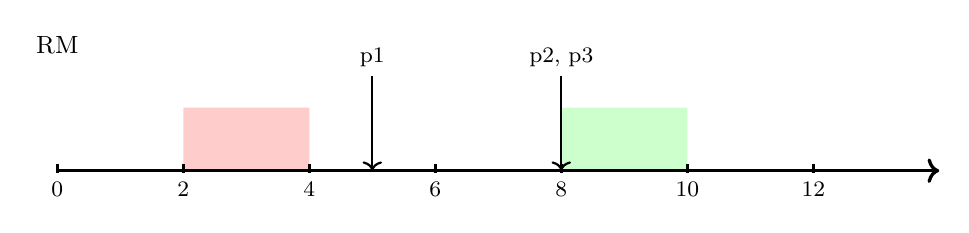
\begin{tikzpicture}[very thick, black, scale=.8]
        \small

        % Title
        \draw ($(0,2)$) node[activity, black] {RM};

        %% Filled regions
        \fill[color=color1!20] rectangle ($(2,0)$) -- ($(4,0)$) -- ($(4,1)$) -- ($(2,1)$);
        \fill[color=color2!20] rectangle ($(8,0)$) -- ($(10,0)$) -- ($(10,1)$) -- ($(8,1)$);

        % Period
        \draw[<-,thick,color=black] ($(5,0)$) -- ($(5,1.5)$) node [above=0pt,align=center,black,font=\fontsize{8}{0}\selectfont] {p1};

        \draw[<-,thick,color=black] ($(8,0)$) -- ($(8,1.5)$) node [above=0pt,align=center,black,font=\fontsize{8}{0}\selectfont] {p2, p3};

        %% Arrow
        \draw[->] ($(0,0)$) -- ($(14,0)$);

        %% Ticks
        \foreach \x in {0,2,...,12} {
                \draw(\x cm,3pt) -- (\x cm,-1pt);
                \draw (\x,0) node[below=0.5pt, font=\fontsize{8}{0}\selectfont] {\x} ;
            }

    \end{tikzpicture}

\end{frame}
\input{build/uber-frames.tex}

\end{document}